Будем считать, что поставщики конкурируют за бюджет на сумму $K_0$ и 
предоставляют школе скидки $\Delta M$ для победы в закупке \cite{shubik1971game}.
 При этом поставщики несут издержки как постоянные $FC$, так и относительные $p$, пропорционально зависящие от бюджета K0. Тогда прибыль поставщика будет равна:
\begin{equation}
    K_0- FC- pK_0- \Delta M =1-p \cdot K_0 -FC- \Delta M   
\end{equation}
Функция полезности поставщика будет являться функцией прибыли, так как основной задачей поставщика будет являться максимизация его прибыли.
\begin{equation}
    U = 
\end{equation}



\begin{figure}[h]
    \centering
    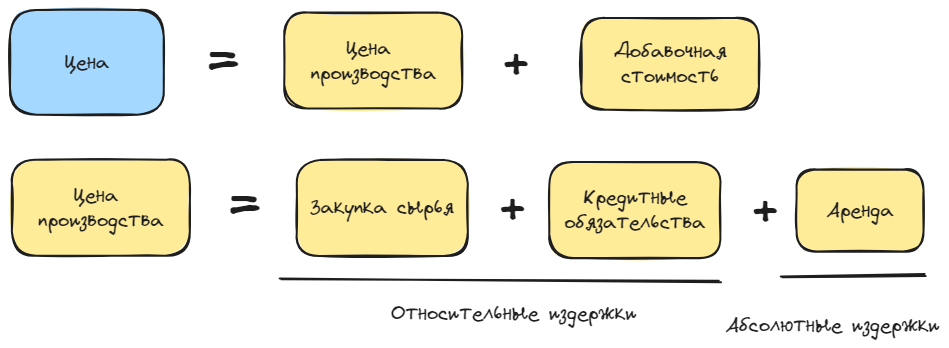
\includegraphics[width=0.5\textwidth]{assets/settings/price_form.excalidraw.png}
    \caption{Формирование цены}
\end{figure}

Определим также базовую функцию $P$ и выручку $TR$ поставщика: 
\begin{equation}
    \begin{cases}
        P=1-p \cdot K_0 -FC  \\
        TR=K_0- \Delta M 
    \end{cases}
\end{equation}

Значение базовой функции зависит от способности поставщика к снижению относительных и постоянных издержек, определяет его конкурентность. В условиях равной скидки поставщик с большим значением базовой функции получит большую прибыль.
Выручка также как и прибыль может быть оптимизируемой функцией для поставщиков - функцией полезности. Малые игроков заключая сделки ориентируются на максимизацию прибыли. Крупные, если сделка приносит неотрицательную прибыль, на максимизацию выручки. Соответственно, для крупных поставщиков функцией полезности будет являться функция выручки. 
малые игроки:
$$
    U= \pi \rightarrow \max \ge 0
$$
крупные игроки: 
$$
    U = \text{TR} \rightarrow \max , \pi \ge 0
$$
В экспертной постановке критерием крупного игрока в Российской Федерации можем считать ежегодную выручку более 400 млн рублей.
В работе \cite{Bogdanov2023} разобран случай закрытого аукциона, в котором значение базовой функции поставщика неизвестна прочим игрокам. В условиях аукциона закупку выигрывает поставщик с наибольшей скидкой на лот. 
При моделировании процесса конкуренции предполагаем, что поставщик предполагает скидки прочих игроков равновероятными. При принятии собственного решения он подбирает скидку, исходя из максимизации математического ожидания полезности. В условиях $n$ поставщиков, где $n=k+m$, где $k$ - число поставщиков, максимизирующих прибыль, а $m$ - число поставщиков, максимизирующих выручку, получаем:

\begin{equation}
    \begin{cases}
        \Delta M_i = P_i \cdot \frac{n-1}{n} 
        \Delta M_i = K_0 \frac{n-1}{n} \text{при}  P_i- K_0*\frac{n-1}{n} \ge 0, \text{иначе} \Delta M_i  P_i 
    \end{cases}
\end{equation}

Заметим, что скидки игроков с ростом числа участников аукциона стремятся к их базовой функции. То есть лоты в условиях закрытого аукциона при достаточном числе участников будут продаваться по себестоимости товара. 
